\graphicspath{{./2-Arquitectura/capitulo5/}}

\Capitulo{Negocio}{

En el tejido empresarial, la Capa de Negocios emerge como el lienzo donde las estrategias se materializan en operaciones tangibles, y donde la agilidad y la eficiencia son la moneda de cambio. Este capitulo se adentra en la Capa de Negocios. \textbf{Este espacio es vital para entender y optimizar los procesos, la estructura organizativa y el valor que la empresa ofrece.
}
A lo largo de estas páginas, exploraremos cada uno de los modelos dentro de la Capa de Negocios, desde la identificación de los actores clave y sus roles hasta la meticulosa descripción de procesos de negocio y la asignación de servicios empresariales. Cada modelo se erige como una pieza fundamental para traducir la estrategia en ejecución efectiva, alineando la estructura organizativa y los recursos con los objetivos de la empresa.

La Capa de Negocios, en este contexto, \textbf{no es solo un espejo de la estrategia, sino un motor que impulsa la creación de valor}. Desde la oferta de productos y servicios hasta la gestión de recursos clave, cada elemento modelado contribuye a la comprensión integral de cómo la organización realiza sus operaciones cotidianas.

Este análisis, arraigado en las mejores prácticas de ADM, busca ser un faro para aquellos que buscan optimizar la eficiencia y la eficacia de sus operaciones comerciales. Haremos este recorrido detallado por la Capa de Negocios para descubrir cómo la arquitectura empresarial se convierte en un aliado estratégico, transformando la visión en resultados tangibles en el complejo paisaje de los negocios.
}

%--------------Organización -----------------------


\newpage
\section{Organización}
\subsection{Modelo}
\begin{figure}[H]
	\centering	
    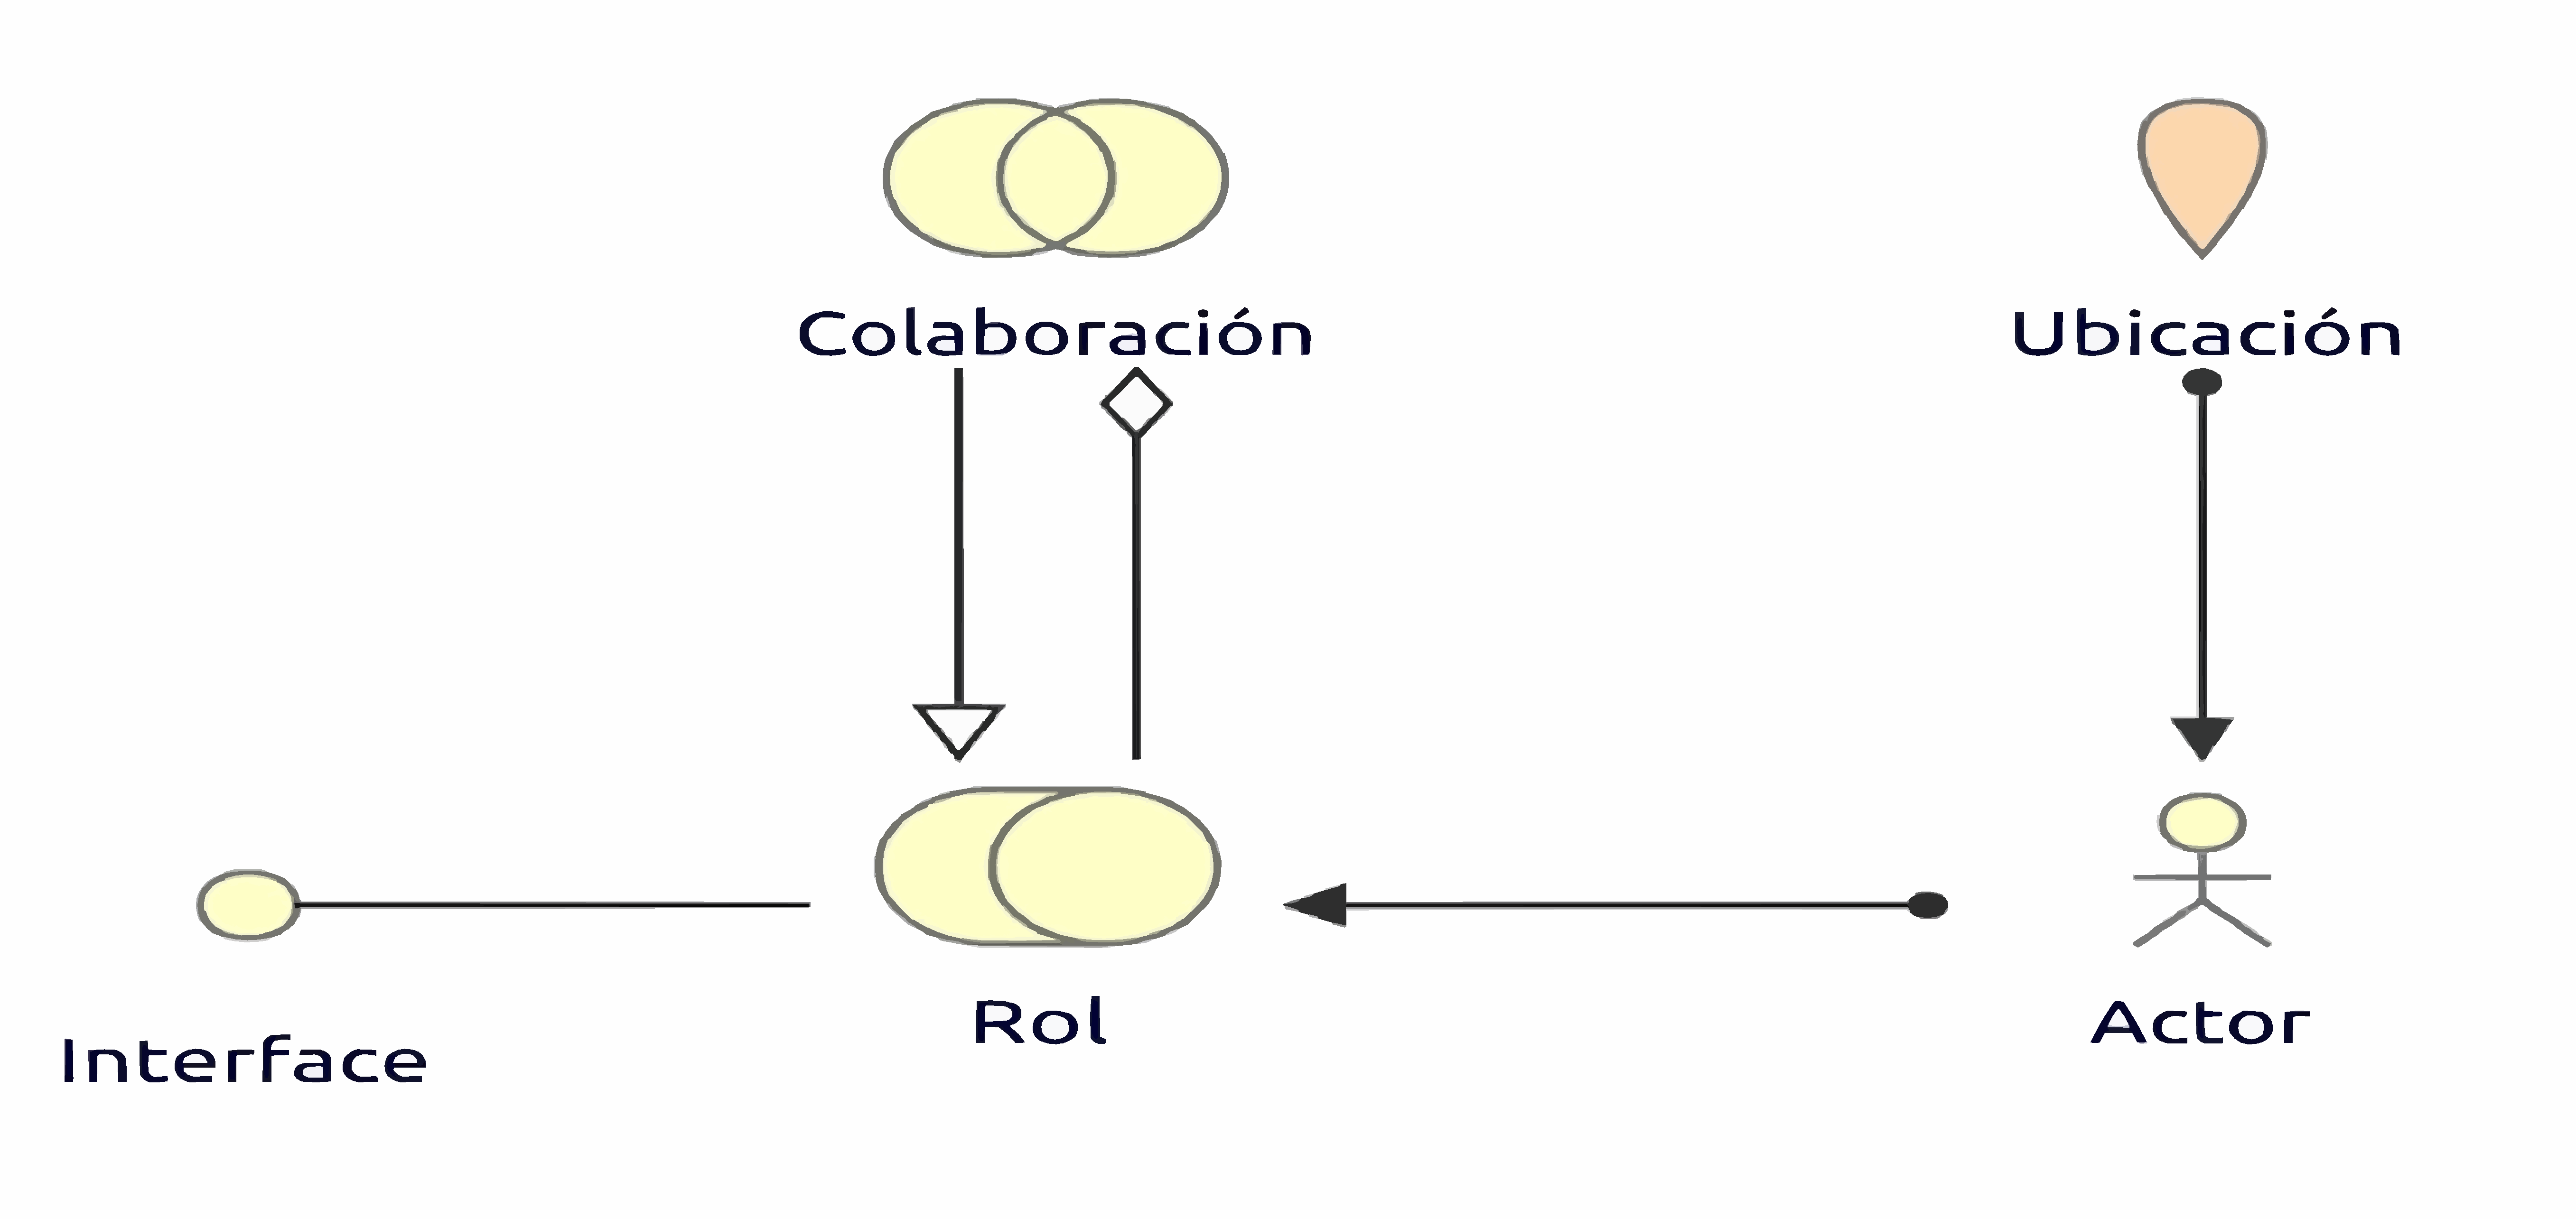
\includegraphics[width=0.7\linewidth]{imgs/OrganizacionM.pdf}
	\caption{Modelo Organización}
\end{figure}
El modelo de organización se utiliza para representar la estructura y relaciones internas de una entidad empresarial. Este modelo ayuda a entender cómo se organizan y se relacionan los diferentes roles, actores y colaboraciones dentro de la empresa. Estos elementos se interconectan para formar la estructura organizativa que soporta la arquitectura de negocio.
\subsection{Caso}
\begin{figure}[H]
	\centering	
    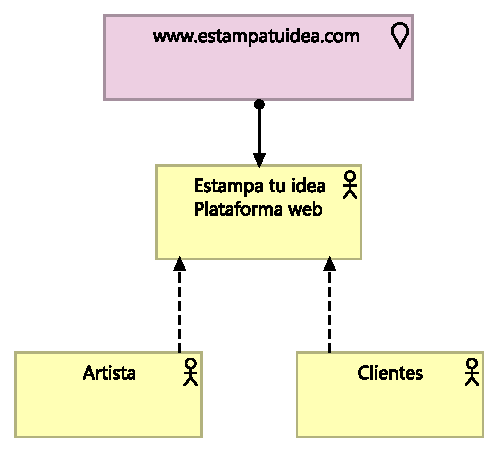
\includegraphics[width=0.55\linewidth]{imgs/Caso 1.pdf}
	\caption{Caso Organización}	
 \end{figure}

     El diagrama ilustra la conexión entre los artistas y los clientes a través de la plataforma web “Estampa tu idea”. Los artistas suben sus diseños a la plataforma, y los clientes pueden navegar y comprar estos diseños.\textbf{ Este enfoque fomenta la creatividad y la personalización, al tiempo que ofrece a los artistas una oportunidad de exponer y vender su trabajo.} Este modelo estratégico ayuda a la organización a diferenciarse en el mercado al proporcionar una experiencia única de personalización y al establecer una conexión directa entre artistas y consumidores. \textbf{Es una estrategia sólida que alinea los objetivos generales y específicos con los principios de la marca, como la creatividad, la calidad, el servicio al cliente, la transparencia y la innovación.}

%--------------Cooperacion de Actor-----------------------
\PuntoDeVista{Cooperación de Actor}{imgs/CooperaciondeActorM.pdf}
{
   Este modelo es crucial para entender cómo diferentes actores colaboran y se interrelacionan dentro de una organización para lograr objetivos comunes.
   
   Estos elementos se conectan para formar una red de cooperación que facilita la realización de actividades de negocio y la consecución de metas estratégicas. Además, se utiliza para analizar y diseñar la forma en que la organización se estructura y cómo se llevan a cabo las interacciones entre los diferentes actores.
}
{imgs/Caso 2.pdf}
{
    Este flujo de interacción refleja la propuesta de valor de Estampa tu idea plasmada en la cooperacion de los roles, conectando la creatividad de los artistas con las preferencias de los clientes para crear productos únicos y personalizados. Los principios de la marca, como la creatividad y la innovación, se ven claramente en este modelo, al igual que el compromiso con la calidad y el servicio al cliente.
}{0.8}{1}

%--------------Función de Negocio-----------------------
\PuntoDeVista{Función de Negocio}{imgs/FunciondeNegocioM.pdf}
{
    Este modelo representa la estructura organizativa y las responsabilidades dentro de una empresa La secuencia de flechas indica el flujo de trabajo desde el actor hasta la función, mostrando cómo un individuo asume un rol y luego ejecuta una función relacionada con ese rol. 

    Este modelo es útil para visualizar y comprender cómo se distribuyen y se llevan a cabo las responsabilidades dentro de una organización, y cómo los individuos interactúan con los procesos de negocio a través de los roles que desempeñan. 
}{imgs/Caso 3.pdf}
{
    Para este caso se evidencia que \textbf{cada uno de los eventos de negocio mostrados están interrelacionados y contribuyen al objetivo general }de proporcionar una experiencia de personalización única y de alta calidad a los clientes, llevado de la mano de los diseñadores que toman el rol de artistas para convertirse en un facor fundamental a la hora de seguir los principios de la empresa.
}{1}{1}

%------------Proceso de Negocio-------------------------
\PuntoDeVista{Proceso de Negocio}{imgs/ProcesodeNegocioyCooperacionM.pdf}{
    La perspectiva de realización de requerimientos involucra objetivos que son la base para su elaboración es decir son aquellos que motivan su realización, este diagrama permite modelarlos y establecer un nivel de detalle más avanzado que permitirá identificar elementos adicionales que se representan como especializaciones que en un principio puede que no se hayan detectado.
}{imgs/Caso 4.png}{
Este caso representa el proceso de negocio relacionado con la venta de camisetas estampadas, desde el pedido inicial y la logística detrás de la validación del pedido hasta la entrega final.
}{1}{0.9}

%----------------Cooperacion de Proceso de Negocio----------------------
\PuntoDeVista{Cooperación de Proceso de Negocio}{imgs/ProcesodeNegocioyCooperacionM.pdf}{
    Este punto de vista permite mostrar los principales elementos motivacionales para el desarrollo del sistema, estos se generan mediante los objetivos de cada uno de los participantes y que al final son traducidos en requerimientos que se deben cumplir para satisfacer las necesidades manifestadas.

}{imgs/Caso 5.png}{
Este caso ilustra cómo los actores colaboran en un proceso de negocio específico. El “Cliente” realiza un pedido, y el “Proveedor” y el o los ``artistas'' cooperan para satisfacer ese pedido desde la recepción hasta la entrega final.
}{1}{1}

%----------------Producto----------------------
\PuntoDeVista{Producto}{imgs/ProductoM.pdf}{
    Este punto de vista ofrece una visión comprehensiva de la dinámica empresarial, destacando elementos como ``Producto'', ``Contrato'' y ``Evento''. Estos se conectan con otros componentes como ``Servicio'' y ``Proceso/Función'', delineando las relaciones y flujos fundamentales en la estructura empresarial.

}{imgs/Caso6.pdf}{
En la representación visual del caso de producto se destaca se destaca el caso de producto ``Venta de camisetas con diseños personalizados'', conectado a elementos como ``Estampa tu Idea'' , ``Diseños Únicos'' , y ``Entrega de productos a tiempo y costo competitivo''. Factores como ``Sugerencias en estampados para camisetas'' y ``Facilidad de Pago'' contribuyen a la mejora continua y la conveniencia del cliente. Este enfoque del proceso central de venta de camisetas personalizadas proporciona una comprensión clara de cómo estos elementos se entrelazan, \textbf{siendo crucial para la optimización y diseño estratégico de procesos, servicios y productos dentro de la organización.}
}{1}{0.9}

